\documentclass{scrartcl}	% classe article di KOMA
\reversemarginpar
\newcommand{\MarginDate}[1]{\marginpar{\raggedleft\itshape\small#1}}
%\usepackage[latin1]{inputenc}	% la codifica di input
%\usepackage[T1]{fontenc}	% la codifica dei font
\usepackage[LabelsAligned]{currvita}	% un buon pacchetto per CV
\usepackage[nochapters]{classicthesis} % stile ClassicThesis
\usepackage{url}	% per gli indirizzi Internet
\renewcommand{\cvheadingfont}{\LARGE\color{Maroon}}
\renewcommand{\cvlistheadingfont}{\large}
\renewcommand{\cvlabelfont}{\qquad}
%Setup hyperref package, and colours for links, text and headings
\usepackage{hyperref}		
\hypersetup{colorlinks,breaklinks,
	    urlcolor=Maroon, 
	    linkcolor=Maroon}
\usepackage{eurosym}
\usepackage{graphicx}
\usepackage{float}
\usepackage{ragged2e}
\newlength{\datebox}\settowidth{\datebox}{Summer 2007}

\newcommand{\NewWorkExperience}[3]{\noindent\hangindent=2em\hangafter=0 \parbox{\datebox}{\textit{#1}}\hspace{1.5em} #2 #3%
\vspace{0.5em}}

\newcommand{\Description}[1]{\hangindent=2em\hangafter=0\noindent\raggedright\footnotesize{#1}\par\normalsize}
\newcommand{\Sep}{\vspace{2em}}
\begin{document}
\thispagestyle{empty}
\begin{cv}{\spacedallcaps{Vojtech Vitek}}

%%% Contact %%%
\vspace{1.5em}
\noindent\spacedlowsmallcaps{Contact}
\vspace{0.5em}

\MarginDate{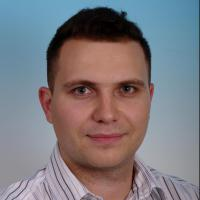
\includegraphics[width=10em]{CV.jpg}}

\NewWorkExperience{E-mail}{\href{mailto:vojtech.vitek@gmail.com}{vojtech.vitek@gmail.com}}{}

\NewWorkExperience{Phone}{+1-647-787-7820}{}

\NewWorkExperience{Location}{Toronto, ON, Canada}{}

\NewWorkExperience{LinkedIn}{\href{http://www.linkedin.com/in/vojtechvitek}{linkedin.com/in/vojtechvitek}}{}

\NewWorkExperience{GitHub}{\href{https://github.com/VojtechVitek}{github.com/VojtechVitek}}{}

\NewWorkExperience{StackOverflow}{\href{http://stackoverflow.com/users/385548/vojtech-vitek}{stackoverflow.com/users/385548/vojtech-vitek}}{}


%%% Summary %%%
%\vspace{1.0em}
%\noindent\spacedlowsmallcaps{Summary}
%\vspace{0.5em}
%
%\Description{\MarginDate{}I'm friendly and positive backend developer who likes traveling and meeting new people. Besides my passion for modern IT technologies, I do several sports actively and I'm also a musician.
%}

%%% Work experience %%%
\vspace{1.5em}
\noindent\spacedlowsmallcaps{Work Experience}
\vspace{0.5em}

\NewWorkExperience{2+ years}{Lead SW Developer at Pressly / Vision Critical}

\Description{\MarginDate{Golang Backend Development Lead}\textit{Feb 2015 - present, Toronto, ON}\newline Leading the backend infrastructure team. Responsible for designing and developing high available Golang REST API microservices. \href{http://www.pressly.com}{www.pressly.com}
\begin{itemize}
  \item Golang, REST, PostgreSQL, Redis, LedisDB, Travis CI
  \item Docker, Ubuntu, EC2
\end{itemize}
Pressly Inc. was acquired by Vision Critical Communications Inc. in July 2017.
}

\Sep

\NewWorkExperience{4.5 years}{Software Engineer at Red Hat}

\Description{\MarginDate{Golang Developer, Docker, Kubernetes}\textit{Aug 2012 - Feb 2015, Brno, Czech Rep.}\newline Developing OpenShift, the next generation PaaS built in Golang on top of Google Kubernetes and Docker containers. Maintaining OpenShift 2 - responsible for Developer Experience and PHP environment (Apache and Zend Server). \href{http://www.openshift.com}{www.openshift.com}
\begin{itemize}
  \item Docker, Kubernetes, RHEL, Atomic, CentOS, Fedora, EC2
  \item Golang, REST, Bash, PHP, Zend Server, MongoDB, Etcd, Jenkins
\end{itemize}
}

\Sep

\Description{\MarginDate{GNU/Linux Software Maintainer}\textit{Oct 2010 - Jul 2012, Brno, Czech Rep.}\newline Fedora/RHEL package maintainer. Responsible for dozen core GNU/Linux applications, most notably PHP 5, PHP PECL extensions, Rsync, GNU Awk, tcsh, gzip, xinetd, less and sed. \href{http://www.redhat.com}{www.redhat.com}
\begin{itemize}
  \item RHEL, Fedora, RPM, Bash, C/C++, PHP 5, Apache, Awk
\end{itemize}
}

\Sep

\NewWorkExperience{5 years}{SysAdmin \& PHP Devel. at Blue Solutions}

\Description{\MarginDate{Linux Sysadmin, Drupal Developer}\textit{2009 - 2013, Brno, Czech Rep.}\newline Side job. Co-founder of dot-com company focusing on robust web portals and e-shops. Responsible for VM-based CentOS server infrastructure. Developing custom Drupal 6/7 modules in PHP 5. \href{http://www.modryweb.cz/}{www.modryweb.cz}
\begin{itemize}
  \item CentOS 6, DNS, Varnish, Nginx, PHP-FPM, OPcache, Redis, MySQL
  \item PHP 5, Drupal 7, Drupal Commerce, JavaScript, jQuery
\end{itemize}
}

\Sep


%%% EDUCATION %%%
\vspace{1.5em}
\noindent\spacedlowsmallcaps{Education}
%\vspace{0.5em}

\NewWorkExperience{2007 - 2011}{Brno University of Technology,}{Czech Rep.}

\Description{\MarginDate{Bachelor's Degree}Information Technology - Bachelor's Degree. Graduated with ``Native Code Browser Extensions'' Bachelor thesis, focused on front-end browser extensions, C/C++ NPAPI plugins for Mozilla Firefox, Google Chrome and Opera browsers and applications sandboxed using Native Client. \newline\newline
\MarginDate{Outstanding Results}Placed in top 5\% students and received several scholarships for outstanding academic results. \href{http://www.fit.vutbr.cz/}{www.fit.vutbr.cz}
\newline\newline
\MarginDate{Exchange~Studies}Erasmus exchange studies at Yildiz Technical University, Istanbul, Turkey, focused on Unix operating systems and Oracle database storage technologies. Gained ``A'' grades in all courses taken and received scholarship for outstanding academic results. \href{http://www.yildiz.edu.tr/en/}{www.yildiz.edu.tr/en/}
\newline\newline
\MarginDate{Network Academy Research}Maintaining software tools and low-level drivers for custom High-speed 100G Network Cards, CentOS/Debian server infrastructure and RPM/DEB packaging. \href{http://www.liberouter.org}{www.liberouter.org}
}


%%% Certifications %%%
\vspace{1.5em}
\noindent\spacedlowsmallcaps{Certifications}
%\vspace{0.5em}

\Description{\begin{itemize}
 \item Red Hat Certified System Administrator (RHCSA), 120-019-294
 \item Red Hat Project Management Academy, 2012
\end{itemize}
}


%%% Awards %%%
\vspace{1.5em}
\noindent\spacedlowsmallcaps{Awards \& International Scholarships}
%\vspace{0.5em}

\Description{\begin{itemize}
 \item 2011, Winner of the CZ.NIC VIP 3 Open-Source Competition
 \item 2010, Winner of the CZ.NIC VIP 2 Open-Source Competition
 \item 2009, Winner of the Student EEICT Academy Project Competition
 \item 2009, Winner of the GE Foundation International Scholarship for the 15 most accomplished students of technical universities in the Central/Eastern Europe
\end{itemize}
}

\enlargethispage{\baselineskip}
\end{cv}
\end{document}
